\section{Bezier Curves}
\label{sec:bezier}

\subsection{General Definition}

The Bernstein polynomial of order $n$ for the function $f(t)$ is defined on the closed interval $[0,1]$ as

\begin{equation}
    B_n(t) = \sum_{i=0}^n f\left(\frac{i}{n}\right){n\choose i} t^i\left(1-t\right)^{n-i}
    \label{eq:bernstein}
\end{equation}

Equation \ref{eq:bernstein} may be rewritten as

\begin{equation}
    B_n(t) = \sum_{i=0}^n f\left(\frac{i}{n}\right) B_i^n(t)
\end{equation}

where the $B_i^n(t)$ are the Bernstein basis polynomials

\begin{align}
    B_i^n(t) = {n\choose i} t^i (1-t)^{n-i} & & \makecell[l]{ i=0,1,2,\ldots,n \\ n=0,1,2,\ldots }
\end{align}

with

\begin{align}
    {n\choose i} = \frac{n!}{i!(n-i)!}
\end{align}

\subsection{Cubic 2D Bezier}

For a 2-dimensional B\'ezier curve $B_n(t)$ with $n+1$ control points $\vec{p_n} = (p_{i,x}, p_{i,y})$ we can define the curve with equations

\begin{align}
    \left.\begin{aligned}
        x(t) &= \sum_{i=0}^n p_{i,x} B_i^n(t) \\
        y(t) &= \sum_{i=0}^n p_{i,y} B_i^n(t)
    \end{aligned}\right.
    & & 0 \leq t \leq 1
\end{align}

By setting $n=3$ the expressions for $x(t)$ and $y(t)$ can be expanded:

\begin{align}
    x(t) &= \sum_{i=0}^3 p_{i,x} {3\choose i} t^i(1-t)^{3-i} \\
         &= p_{0,x}(1-t)^3 + 3p_{1,x}t(1-t)^2 + 3p_{2,x}t^2(1-t) + p_{3,x}t^3 \\
         &= p_{0,x}(1-3t+3t^2-t^3) + p_{1,x}(3t-6t^2+3t^3) + p_{2,x}(3t^2-3t^3) + p_{3,x}t^3 \\
         &= p_{0,x} + (-3p_{0,x} +3p_{1,x})t + (3p_{0,x} -6p_{1,x} +3p_{2,x})t^2 + (-p_{0,x}+3p_{1,x}-3p_{2,x}+p_{3,x})t^3
\end{align}

and finally re-arranged into 3rd order polynomials:

\begin{align}
    x(t) &= a_{0,x} + a_{1,x} t + a_{2,x} t^2 + a_{3,x} t^3 \label{eq:bezier_x} \\
    y(t) &= a_{0,y} + a_{1,y} t + a_{2,y} t^2 + a_{3,y} t^3 \label{eq:bezier_y}
\end{align}

where the polynomial coefficiants $a_{0,x} \ldots a_{3,x}$ and $a_{0,y} \ldots a_{3,y}$ are:

\begin{align}
    \begin{bmatrix}
        a_{0,x} & a_{0,y} \\
        a_{1,x} & a_{1,y} \\
        a_{2,x} & a_{2,y} \\
        a_{3,x} & a_{3,y}
    \end{bmatrix}
    &=
    \left[\begin{array}{ll}
        p_{0,x}                                   & p_{0,y} \\
        -3p_{0,x} + 3p_{1,x}                      & -3p_{0,y} + 3p_{1,y} \\
        3p_{0,x}  - 6p_{1,x} + 3p_{2,x}           & 3p_{0,y}  - 6p_{1,y} + 3p_{2,y} \\
        -p_{0,x}  + 3p_{1,x} - 3p_{2,x} + p_{3,x} & -p_{0,y}  + 3p_{1,y} - 3p_{2,y} + p_{3,y}
    \end{array}\right]
\end{align}

Notice that the coefficients of the two polynomials $x(t)$ and $y(t)$ are independent of one another. The problem of fitting the curve to data becomes much easier as a result.

\subsection{Polynomial Regression}
\label{sec:polynomial-regression}

As the snake head moves forward in time, it leaves behind a list of $m$ number of 2D data points $(x_i,y_i)$. We can make the reasonable assumption these are distributed along a bezier curve $x(t),y(t)$ with $t\in[0..1]$. The problem is then to find suitable coefficients $a_{0,x} \ldots a_{3,x}$ and $a_{0,y} \ldots a_{3,y}$ for the polynomial regression models

\begin{align}
    x_i &= a_{0,x} + a_{1,x} t_i + a_{2,x} t_i^2 + \ldots + a_{n,x} t_i^n + \epsilon_i \\
    y_i &= a_{0,y} + a_{1,y} t_i + a_{2,y} t_i^2 + \ldots + a_{n,y} t_i^n + \epsilon_i
    \label{eq:regression-models}
\end{align}

These can be expressed in matrix form in terms of a design matrix $T$, a response matrix $X$, a parameter matrix $A$ and a matrix $\epsilon$ of random errors. The $i$-th row of $T$ and $X$ will contain the $t$ and $(x,y)$ value of the $i$-th data sample. Then the model can be written as a system of linear equations:

\begin{align}
    \begin{bmatrix}
        x_1 & y_1 \\ x_2 & y_2 \\ \vdots & \vdots \\ x_m & y_m
    \end{bmatrix}
    &=
    \begin{bmatrix}
        1      & t_1     & t_1^2     & \ldots & t_1^n \\
        1      & t_2     & t_2^2     & \ldots & t_2^n \\
        \vdots & \vdots  & \vdots    & \ddots & \vdots \\
        1      & t_m     & t_m^2     & \ldots & t_m^n
    \end{bmatrix}
    \begin{bmatrix}
        a_{0,x} & a_{0,y} \\
        a_{1,x} & a_{0,y} \\
        \vdots  & \vdots \\
        a_{n,x} & a_{n,y}
    \end{bmatrix}
    +
    \begin{bmatrix}
        \epsilon_{1,x} & \epsilon_{1,y} \\
        \epsilon_{2,x} & \epsilon_{2,y} \\
        \vdots         & \vdots \\
        \epsilon_{m,x} & \epsilon_{m,y}
    \end{bmatrix}
    \label{eq:regression-model}
\end{align}

The coefficients matrix $A$ can be calculated using ordinary least squares estimation:

\begin{equation}
    A = (T^T T)^{-1} T^T X
    \label{eq:olse}
\end{equation}

\subsection{Constrained Polynomial Regression}

One issue with using equation \ref{eq:olse} directly is that as new curve segments are created, the ends of the individual bezier curves will not line up correctly, as can be seen in figure \ref{fig:bezier_fit}.

\begin{figure}
    \centering
    \begin{subfigure}{.45\linewidth}
        \centering
        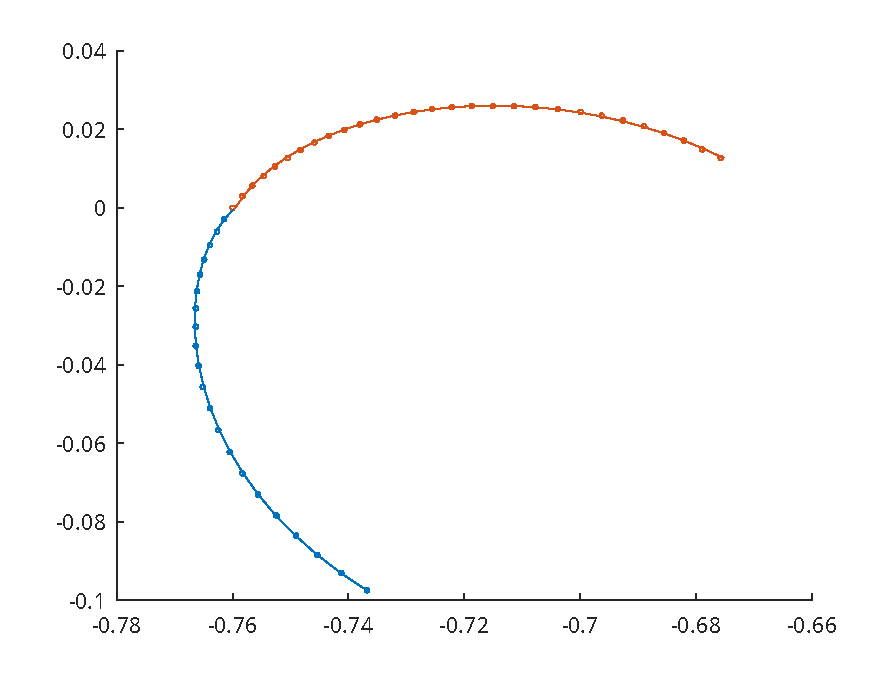
\includegraphics[width=\linewidth]{bezier_fit.pdf}
        \caption{}
    \end{subfigure}
        \begin{subfigure}{.45\linewidth}
        \centering
        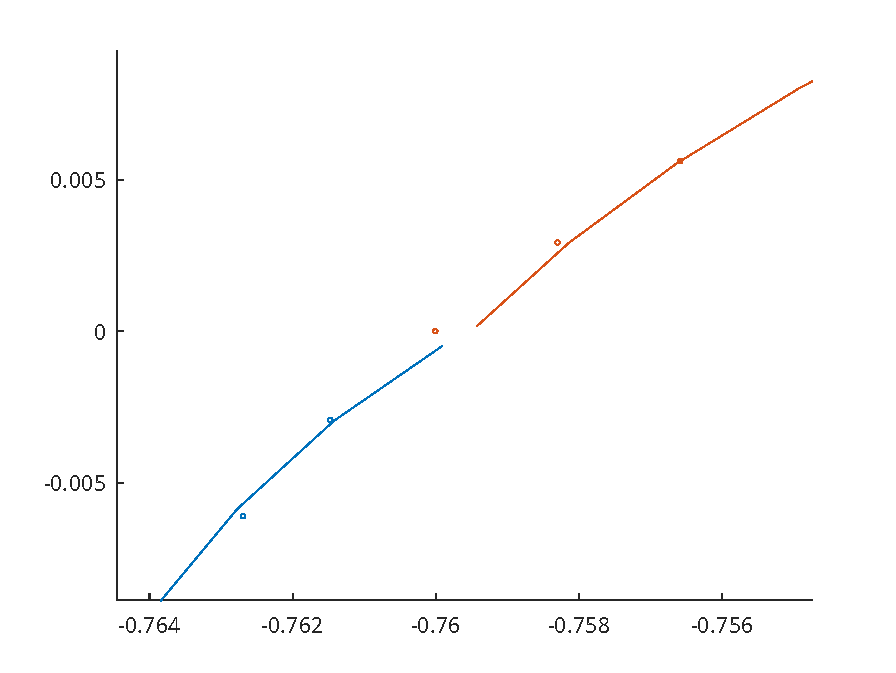
\includegraphics[width=\linewidth]{bezier_fit_zoom.pdf}
        \caption{}
    \end{subfigure}
    \caption{Two bezier curves fitted to points using polynomial regression.\\The ends do not meet.}
    \label{fig:bezier_fit}
\end{figure}

It is necessary to constrain the regression model such that the curve always passes through the start and end points of the input data.

Following an answer on stackexchange\cite{web:constrained-regression}, equations \ref{eq:regression-models} can be reformulated as:

\begin{align}
    x(t) &= f_x(t) + (t-t_1)\ldots(t-t_d)(b_{0,x} + b_{1,x} t + \ldots + b_{n-d,x} t^{n-d}) \\
    y(t) &= f_y(t) + (t-t_1)\ldots(t-t_d)(b_{0,y} + b_{1,y} t + \ldots + b_{n-d,y} t^{n-d})
\end{align}

where $d$ is the number of points to constrain, $t_1 \ldots t_d$ are the specific data points to constrain (corresponding with $(x_i,y_i)$) -- note here that they do not need to be in sequence. $fx(t)$ and $fy(t)$ are polynomials of degree $d-1$ that must pass through all constrained data points $(t_i,x_i,y_i)$, and $b_{i,x}$ and $b_{i,y}$ are the coefficients to solve for.

Notice that the degree of the polynomial decreases for every point constrained.

In our case we want to constrain the first and last data points $(t_1,x_1,y_1)$ and $(t_m,x_m,y_m)$. By defining

\begin{equation}
    r(t) = (t-t_1)(t-t_m)
\end{equation}

the problem can be rewritten as

\begin{align}
    x(t) - f_x(t) &= r(t) b_{0,x} + r(t) b_{1,x} t \label{eq:cpr1x} \\
    y(t) - f_y(t) &= r(t) b_{0,y} + r(t) b_{1,y} t \label{eq:cpr1y}
\end{align}

which is a standard ordinary least squares estimation problem that can be solved using the equations in section \ref{sec:polynomial-regression}.

A problem that occurred during development, though, is that the values in the $(T^T T)^{-1} T^T$ matrix in general differed in orders of magnitudes from the data points and coefficients. This is a problem because these algorithms are implemented using fixed-point arithmetic in clither, and the precision of multiplication and division operations directly depends on the differences in magnitudes of the values involved. In many cases the matrix would end up containing $0$ because the values were too small to represent with the fixed-point type.

For this reason, equations \ref{eq:cpr1x} and \ref{eq:cpr1y} are re-arranged to:

\begin{align}
    \frac{x(t) - f_x(t)}{r(t)} &= b_{0,x} + b_{1,x} t \\
    \frac{y(t) - f_y(t)}{r(t)} &= b_{0,y} + b_{1,y} t
\end{align}

This removes $r(t)$ as a factor in the $T$ matrix and improves the precision issues.

Notice, however, that $r(t)$ has a singularity at $t_1$ and $t_m$, and therefore, the $T$ matrix must be built excluding those data points.

The functions $f_x(t)$ and $f_y(t)$ in this case are linear functions, since $d=2$, and must pass through data points $(t_1,x_1,y_1)$ and $(t_m,x_m,y_m)$ respectively.

\begin{align}
    f_x(t) &= m_x t + q_x & \text{where} && m_x = \frac{x_m-x_1}{t_m-t_1} &,& q_x &= x_1 \\
    f_y(t) &= m_y t + q_y & \text{where} && m_y = \frac{y_m-y_1}{t_m-t_1} &,& q_y &= y_1
\end{align}

The coefficients $b_{0,x}, b_{0,y}, b_{1,x}, b_{1,y}$ can now be calculated by creating a system of linear equations following \ref{eq:regression-model}:

\begin{align}
    \begin{bmatrix}
        \frac{x_2 - f_x(t_2)}{r(t_2)} & \frac{y_2 - f_x(t_2)}{r(t_2)} \\
        \frac{x_3 - f_y(t_3)}{r(t_3)} & \frac{y_3 - f_y(t_3)}{r(t_3)} \\
        \vdots & \vdots \\
        \frac{x_{m-1} - f_x(t_{m-1})}{r(t_{m-1})} & \frac{y_{m-1} - f_y(t_{m-1})}{r(t_{m-1})}
    \end{bmatrix}
    &=
    \begin{bmatrix}
        1      & t_1     \\
        1      & t_2     \\
        \vdots & \vdots  \\
        1      & t_m
    \end{bmatrix}
    \begin{bmatrix}
        b_{0,x} & b_{0,y} \\
        b_{1,x} & b_{1,y}
    \end{bmatrix}
    +
    \begin{bmatrix}
        \epsilon_{2,x} & \epsilon_{2,y} \\
        \epsilon_{3,x} & \epsilon_{3,y} \\
        \vdots         & \vdots \\
        \epsilon_{x,{m-1}} & \epsilon_{y,{m-1}}
    \end{bmatrix}
\end{align}

and solved using equation \ref{eq:olse}.

The control points $p_{0,x} \ldots p_{3,x}$ and $p_{0,y} \ldots p_{3,y}$ of the cubic bezier curve can be recovered from $b_{0,x},b_{1,x}$ and $b_{0,y},b_{1,y}$ by comparing coefficients of the two polynomial equations.

Equations \ref{eq:cpr1x} and \ref{eq:cpr1y} expanded and re-arranged:

\begin{align}
    x(t) &= q_x + (m_x - b_{x,0}) t + (b_{x,0} - b_{x,1}) t^2 + b_{x,1} t^3 \\
    y(t) &= q_y + (m_y - b_{y,0}) t + (b_{y,0} - b_{y,1}) t^2 + b_{y,1} t^3
\end{align}

Equations \ref{eq:bezier_x} and \ref{eq:bezier_y} expanded and re-arranged:

\begin{align}
    x(t) &= p_{0,x} + (-3p_{0,x} + 3p_{1,x})t + (3p_{0,x} - 6p_{1,x} + 3p_{2,x})t^2 + (-p_{0,x} + 3p_{1,x} - 3p_{2,x} + p_{3,x})t^3 \\
    y(t) &= p_{0,y} + (-3p_{0,y} + 3p_{1,y})t + (3p_{0,y} - 6p_{1,y} + 3p_{2,y})t^2 + (-p_{0,y} + 3p_{1,y} - 3p_{2,y} + p_{3,y})t^3
\end{align}

By comparing the coefficients of these equations, the control points can be calculated:

\begin{align}
    q_x               &= p_{0,x}              &
    p_{0,x} &= q_x \\
    m_x - b_{0,x}     &= -3p_{0,x} + 3p_{1,x} &
    p_{1,x} &= \frac{1}{3} (m_x - b_{0,x} + 3p_{0,x}) \\
    b_{0,x} - b_{1,x} &= 3p_{0,x} - 6p_{1,x} + 3p_{2,x} &
    p_{2,x} &= \frac{1}{3} (b_{0,x} - b_{1,x} - 3p_{0,x} + 6p_{1,x}) \\
    b_{1,x}           &= -p_{0,x} + 3p_{1,x} - 3p_{2,x} + p_{3,x} &
    p_{3,x} &= b_{1,x} + p_{0,x} - 3p_{1,x} + 3p_{2,x}
\end{align}

\begin{align}
    q_x               &= p_{0,y}              &
    p_{0,y} &= q_x \\
    m_x - b_{0,y}     &= -3p_{0,y} + 3p_{1,y} &
    p_{1,y} &= \frac{1}{3} (m_x - b_{0,y} + 3p_{0,y}) \\
    b_{0,y} - b_{1,y} &= 3p_{0,y} - 6p_{1,y} + 3p_{2,y} &
    p_{2,y} &= \frac{1}{3} (b_{0,y} - b_{1,y} - 3p_{0,y} + 6p_{1,y}) \\
    b_{1,y}           &= -p_{0,y} + 3p_{1,y} - 3p_{2,y} + p_{3,y} &
    p_{3,y} &= b_{1,y} + p_{0,y} - 3p_{1,y} + 3p_{2,y}
\end{align}

\begin{figure}
    \centering
    \begin{subfigure}{.45\linewidth}
        \centering
        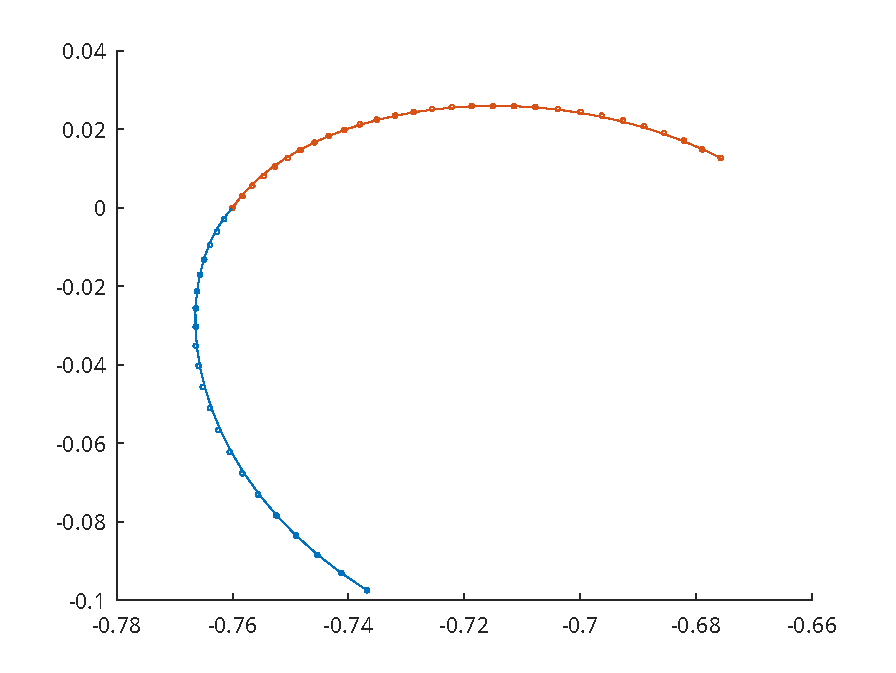
\includegraphics[width=\linewidth]{constrained_bezier_fit.pdf}
        \caption{}
    \end{subfigure}
        \begin{subfigure}{.45\linewidth}
        \centering
        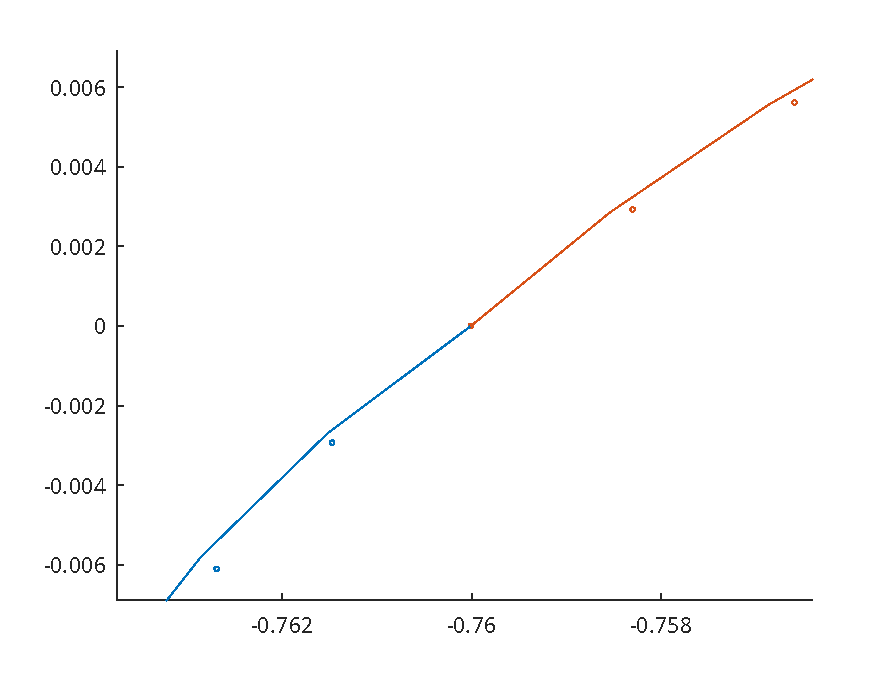
\includegraphics[width=\linewidth]{constrained_bezier_fit_zoom.pdf}
        \caption{}
    \end{subfigure}
    \caption{Two bezier curves fitted using constrained polynomial regression.\\The ends now meet.}
    \label{fig:constrained_bezier_fit}
\end{figure}

\clearpage
\subsection{Axis-Aligned Bounding Box}

\begin{figure}
    \centering
    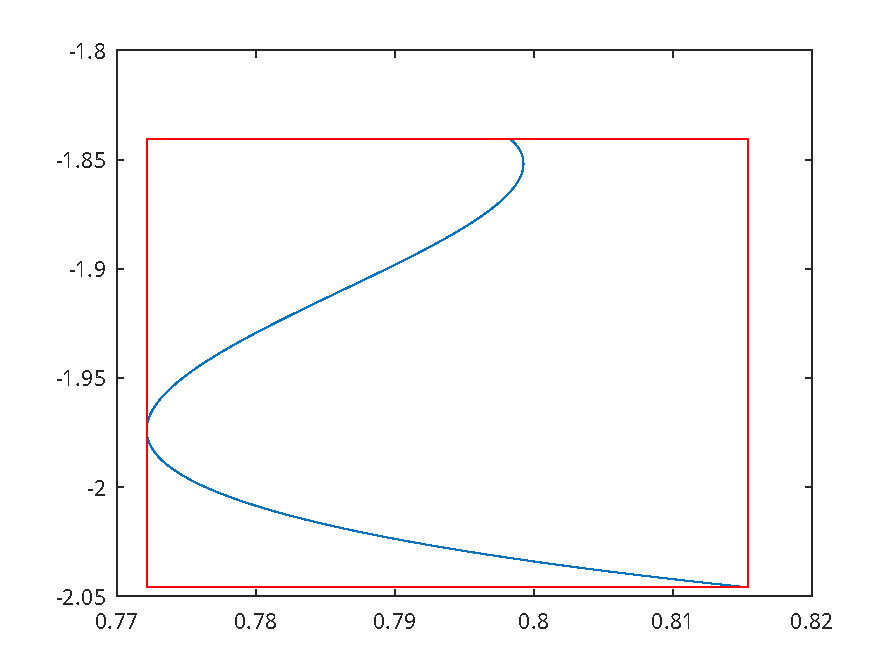
\includegraphics[width=.45\linewidth]{aabb.pdf}
    \caption{Bounding box of a cubic bezier curve.}
    \label{fig:bezier_aabb}
\end{figure}

In order to speed up collision checks, the axis-aligned bounding box (AABB) is calculated for each curve segment.

There are $4$ coordinates in total that define the extremities of the bounding box: $(x_0,y_0) \ldots (x_3,y_3)$.

$(x_0,y_0)$ and $(x_3,y_3)$ are the easiest to calculate, they are simply the start and end points of the curve:

\begin{align}
    x_0 &= x(0) & y_0 &= y(0) \\
    x_3 &= x(1) & y_3 &= y(1)
\end{align}

As can be seen in figure \ref{fig:bezier_aabb}, the AABB formed by the start and end points doesn't always encapsulate the entire curve. By finding the roots of the derivatives:

\begin{align}
    x'(t) &= a_{1,x} + 2 a_{2,x} t + 3 a_{3,x} t^2 \\
    y'(t) &= a_{1,y} + 2 a_{2,y} t + 3 a_{3,y} t^2
\end{align}

\begin{align}
    {t_{0,x},t_{1,x}} &= \frac{-2 a_{2,x} \pm\sqrt{4a_{2,x}^2 - 12 a_{1,x} a_{3,x}}}{2 a_{1,x}} \\
    {t_{0,y},t_{1,y}} &= \frac{-2 a_{2,y} \pm\sqrt{4a_{2,y}^2 - 12 a_{1,y} a_{3,y}}}{2 a_{1,y}}
\end{align}

the AABB can be updated to include these new extremities (if the roots exist and are indeed in the range $[0..1]$)

\begin{align}
    x_1 &= x(t_{0,x}) & \text{if} && 0 \le t_{0,x} \le 1 &,& y_1 &= y(t_{0,y}) & \text{if} && 0 \le t_{0,y} \le 1 \\
    x_2 &= x(t_{1,x}) & \text{if} && 0 \le t_{1,x} \le 1 &,& y_2 &= y(t_{1,y}) & \text{if} && 0 \le t_{1,y} \le 1
\end{align}

\subsubsection{Existence of Complex Roots}

The question arose whether the roots of the derivative of a cubic bezier curve are always real. That is, $4 a_{2,x}^2 - 12 a_{1,x} a_{3,x} \ge 0$? The coefficients $a_{1,x} \ldots a_{3,x}$ depend on the control points $p_{0,x} \ldots p_{3,x}$. For simplicity's sake, we will refer to these control points as $p_0 \ldots p_3$, since finding an answer for the X axis will also be true for the Y axis. Substituting the control points into the inequality yields:

\begin{equation}
    36 \left(-p_0p_2 + p_0p_3 + p_1^2 - p_1p_2 - p_1p_3 + p_2^2\right) \ge 0
    \label{eq:sqrt-inequality}
\end{equation}

It can be shown that equation \ref{eq:sqrt-inequality} is false for all values of $p_0 \ldots p_3$ with the following constraints applied:

\begin{equation}
    \left.
    \begin{array}{ll}
        p_0 &= -\frac{-z_0^2 + z_0z_1 + z_0z_2 - z_1^2 + z_3}{z_1 - z_2} \\
        p_1 &= z_0 \\
        p_2 &= z_1 \\
        p_3 &= z_2
    \end{array}
    \right\}\text{$z_1 \ne z_2$ and $0 \le z_3$}
\end{equation}
